% Common preamble for PIGMIE patent figures (A4).
% Drawing conventions:
%   - A4 portrait
%   - Sans-serif throughout (Helvetica)
%   - "Fig. N" sentence-case caption near top
%   - Page "N/total" at top centre
%   - Reference numerals outside boxes via leader lines
%   - ALL CAPS labels in component boxes
%   - Reactor uses north-east-lines hatched fill
%   - Scene uses double-line border
%   - Module enclosures use dashed line with internal numeral

\documentclass[a4paper,10pt]{article}
\usepackage[top=2.5cm,bottom=1.0cm,left=2.5cm,right=1.5cm]{geometry}
\usepackage[T1]{fontenc}
\usepackage{helvet}
\renewcommand{\familydefault}{\sfdefault}
\usepackage{amsmath,amssymb,bm}
\usepackage{tikz}
\usetikzlibrary{shapes,shapes.geometric,shapes.misc,arrows.meta,positioning,fit,calc,backgrounds,decorations.pathreplacing,decorations.markings,patterns}
\pagestyle{empty}
\setlength{\parindent}{0pt}

\tikzset{
  % Component box: ALL CAPS label inside, no numeral inside
  cbox/.style={draw, rectangle, minimum height=1.0cm, minimum width=2.4cm,
               align=center, line width=0.5pt, font=\small},
  cbox-tall/.style={cbox, minimum height=1.6cm},
  cbox-wide/.style={cbox, minimum width=3.0cm},
  cbox-narrow/.style={cbox, minimum width=1.8cm, font=\footnotesize},
  % Reactor / physical medium: hatched fill
  reactor/.style={cbox, pattern=north east lines, pattern color=black!70},
  % Scene: double-line border
  scenebox/.style={cbox, double, double distance=1.2pt, line width=0.4pt},
  % Module / sub-module enclosure
  enclosure/.style={draw, rectangle, dashed, line width=0.4pt, inner sep=10pt, rounded corners=2pt},
  enclosure-solid/.style={draw, rectangle, line width=0.5pt, inner sep=10pt, rounded corners=2pt},
  % Arrows
  flowarr/.style={-Latex, line width=0.5pt, font=\scriptsize},
  flowbi/.style={Latex-Latex, line width=0.5pt, font=\scriptsize},
  flowarr-fb/.style={-Latex, line width=0.5pt, dashed, font=\scriptsize},
  % Reference numeral leader-line endpoint and label
  refnum/.style={font=\footnotesize, inner sep=1pt},
  leader/.style={line width=0.4pt, -Latex},
  % Caption banner
  figcap/.style={font=\bfseries\large}
}

% Helper: figure header (page number + Fig. N caption)
\newcommand{\figheader}[3]{%
  % #1 = page number (e.g. "1"), #2 = total pages, #3 = figure label (e.g. "1" or "4A")
  \noindent\hfill\small #1/#2\hfill\null\par
  \vspace{0.2cm}
  \begin{center}\bfseries Fig.\ #3\end{center}
  \vspace{0.2cm}
}


\begin{document}

\figheader{1}{7}{1}

\begin{center}
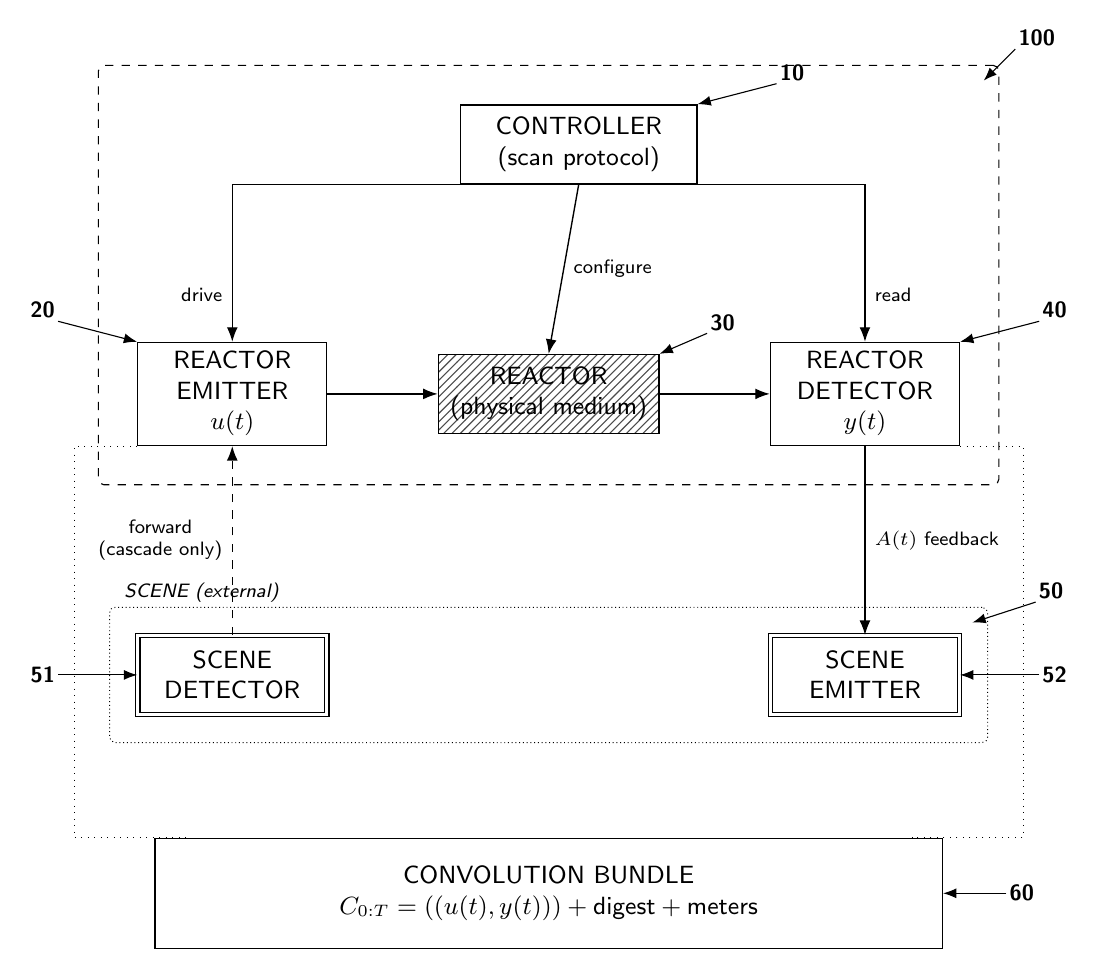
\begin{tikzpicture}[node distance=8mm]

% ============== TOP: Controller ==============
\node[cbox-wide] (ctrl) {CONTROLLER\\(scan protocol)};

% ============== MIDDLE: device-internal signal path ==============
\node[cbox, below=20mm of ctrl, xshift=-44mm, align=center] (re) {REACTOR\\EMITTER\\$u(t)$};
\node[reactor, right=14mm of re, minimum width=2.8cm, align=center] (react)
  {REACTOR\\(physical medium)};
\node[cbox, right=14mm of react, align=center] (rd) {REACTOR\\DETECTOR\\$y(t)$};

% Module 100 enclosure — wraps controller + reactor emitter + reactor + reactor detector
\begin{scope}[on background layer]
  \node[enclosure, fit=(ctrl)(re)(react)(rd), inner sep=14pt] (mod) {};
\end{scope}

% ============== BELOW MODULE: external scene with its own detector/emitter pair ==============
% Scene detector positioned beneath reactor emitter (so the SD -> RE coupling is a clean vertical)
% Scene emitter  positioned beneath reactor detector (so the RD -> SE coupling is a clean vertical)
\node[scenebox, below=24mm of re, minimum width=2.4cm, align=center] (sd)
  {SCENE\\DETECTOR};
\node[scenebox, below=24mm of rd, minimum width=2.4cm, align=center] (se)
  {SCENE\\EMITTER};

% Light-dotted enclosure for SCENE 50 region
\begin{scope}[on background layer]
  \node[draw, rectangle, line width=0.35pt, densely dotted, rounded corners=2pt,
        inner sep=10pt, fit=(sd)(se)] (scene) {};
\end{scope}
\node[font=\scriptsize\itshape, anchor=south west] at ($(scene.north west)+(2pt,-2pt)$)
  {SCENE (external)};

% ============== BOTTOM: convolution bundle ==============
\node[cbox-wide, below=12mm of scene, minimum width=10cm, minimum height=1.4cm] (bundle)
  {CONVOLUTION BUNDLE\\$C_{0:T} = ((u(t),y(t))) + \text{digest} + \text{meters}$};

% ============== Drive / configure / read arrows from controller ==============
\draw[flowarr] (ctrl.south) -| node[pos=0.85, left, font=\scriptsize] {drive} (re.north);
\draw[flowarr] (ctrl.south) -- node[right, font=\scriptsize] {configure} (react.north);
\draw[flowarr] (ctrl.south) -| node[pos=0.85, right, font=\scriptsize] {read} (rd.north);

% ============== Internal forward signal path within module ==============
\draw[flowarr] (re.east) -- (react.west);
\draw[flowarr] (react.east) -- (rd.west);

% ============== Cross-couplings between device and scene ==============
% A(t) feedback: reactor detector -> scene emitter. PRESENT IN BOTH
% embodiments (parallel-subsystem and cascade). Solid arrow.
\draw[flowarr] (rd.south) --
  node[right, font=\scriptsize, pos=0.5] {$A(t)$ feedback}
  (se.north);
% Forward low-latency coupling: scene detector -> reactor emitter.
% CASCADE EMBODIMENT ONLY; omitted in parallel-subsystem embodiment.
% Dashed (flowarr-fb) to flag optionality.
\draw[flowarr-fb] (sd.north) --
  node[left, font=\scriptsize, pos=0.5, align=center] {forward\\(cascade only)}
  (re.south);

% ============== Bundle record (dotted u(t), y(t) lines) ==============
% Routed FAR outside the scene region so they don't graze the scene boxes
\coordinate (uTrack) at ($(re.south west)+(-8mm,0)$);
\coordinate (yTrack) at ($(rd.south east)+(8mm,0)$);
\draw[line width=0.35pt, dotted] (re.south west) -- (uTrack) |- ($(bundle.north west)+(4mm,0)$);
\draw[line width=0.35pt, dotted] (rd.south east) -- (yTrack) |- ($(bundle.north east)+(-4mm,0)$);

% ============== Reference numerals ==============
\node[refnum, anchor=south west] at ($(mod.north east)+(2mm,2mm)$) (n100) {\textbf{100}};
\draw[leader] (n100.south west) -- ($(mod.north east)+(-2mm,-2mm)$);

\node[refnum] at ($(ctrl.north east)+(12mm,4mm)$) (n10) {\textbf{10}};
\draw[leader] (n10.south west) -- (ctrl.north east);

\node[refnum] at ($(re.north west)+(-12mm,4mm)$) (n20) {\textbf{20}};
\draw[leader] (n20.south east) -- (re.north west);

\node[refnum] at ($(react.north east)+(8mm,4mm)$) (n30) {\textbf{30}};
\draw[leader] (n30.south west) -- (react.north east);

\node[refnum] at ($(rd.north east)+(12mm,4mm)$) (n40) {\textbf{40}};
\draw[leader] (n40.south west) -- (rd.north east);

% Scene region numeral 50
\node[refnum] at ($(scene.north east)+(8mm,2mm)$) (n50) {\textbf{50}};
\draw[leader] (n50.south west) -- ($(scene.north east)+(-2mm,-2mm)$);

% Scene detector 51
\node[refnum] at ($(sd.west)+(-12mm,0)$) (n51) {\textbf{51}};
\draw[leader] (n51.east) -- (sd.west);

% Scene emitter 52
\node[refnum] at ($(se.east)+(12mm,0)$) (n52) {\textbf{52}};
\draw[leader] (n52.west) -- (se.east);

\node[refnum] at ($(bundle.east)+(10mm,0)$) (n60) {\textbf{60}};
\draw[leader] (n60.west) -- (bundle.east);

\end{tikzpicture}
\end{center}

\end{document}
